\section{Results}
\label{sec:results}

Tables and figures marked S are in the supplementary material.


\subsection{The tested physics losses and masks do nothing; same-event splits hide the input gain}
\label{sec:loeo}

We first hold out each of the 11 Sen1Floods11 events in turn (Table~S1). The physics losses change
held-out IoU by less than 0.007, because trained models already respect the constraints: without any
physics loss they violate HAND monotonicity on only 0.2--0.5\% of pixel pairs. The first monotonicity loss
compared 4-neighbours at 10\,m, but HAND is a 30-m product resampled to 10\,m, so only 9\% of neighbour
pairs differ by the 1\,m needed to qualify and the loss term stayed near $3\cdot10^{-4}$. Comparing pixels
three apart (one HAND cell; 27\% of pairs qualify), with no margin and weight 1 or 10, the loss engages
(weighted term 0.002--0.013 at the end of training) and cuts the violation rate (weight 10: SAR + HAND
0.0022 → 0.0011, SAR only 0.0041 → 0.0029), yet held-out IoU does not move (−0.001 \ci{−0.006}{+0.004}).
The null is not an implementation artefact. The HAND post-mask changes mean held-out IoU by less than
0.003 for every variant (at most +0.015 on a single event), because models rarely predict flood above
15\,m HAND anyway.

HAND as an input helps a little in LOEO: +0.018 \ci{−0.000}{+0.035} with 3 seeds and +0.025
\ci{+0.005}{+0.045} with 5 (0.566 → 0.591), improving 8 of 11 events. In LOEO the gain sits almost entirely in
the 0--1\,m HAND band, where 75--99\% of each event's flood lies: HAND helps the model place flood within
low ground (on the external events it also removes false alarms on higher ground; Section~\ref{sec:transfer}). One loss is consistent: Somalia, flat
and arid, where every pixel is within a few metres of drainage, so HAND carries no information and
pushes the model toward flood everywhere.

The usual Sen1Floods11 evaluation hides this effect (Fig.~\ref{fig:overview}a). On the official split,
whose test tiles come from the training events, HAND adds +0.007 ± 0.008 pooled IoU (0.671 → 0.679; mean
± standard deviation over 3 seeds); on its Bolivia hold-out, an event absent from training, it adds
+0.128 ± 0.072 (0.556 → 0.685; per seed +0.160, +0.046, +0.179). Bolivia is a single event, but the
contrast is the motivation for this study in miniature: an in-event split measures a different quantity
from transfer to a new flood (the external test below also changes dataset; Section~\ref{sec:discussion}). Eleven events are too few to resolve the LOEO gain precisely; the next
section tests on 79 external events.

\subsection{Transfer to 79 unseen events: HAND helps clearly}
\label{sec:transfer}

\begin{table}[t]
\caption{Trained on all 11 Sen1Floods11 events (3 seeds), tested on GEOID-Flood test. Mean event IoU;
paired Δ with 95\% CI over events; Wilcoxon $p$.}
\label{tab:transfer}
\centering
\footnotesize
\setlength{\tabcolsep}{2.5pt}
\resizebox{\columnwidth}{!}{%
\begin{tabular}{@{}llcccc@{}}
\toprule
Model & Labels & IoU & Δ (95\% CI) & $p$ & Improved \\
\midrule
U-Net & all water & 0.574 → 0.635 & +0.061 [+0.043, +0.080] & $<10^{-4}$ & 69/79 \\
U-Net & flood only & 0.317 → 0.349 & +0.032 [+0.019, +0.047] & $<10^{-4}$ & 57/77 \\
ResNet-34 & all water & 0.581 → 0.618 & +0.036 [+0.018, +0.056] & $<10^{-4}$ & 55/79 \\
ResNet-34 & flood only & 0.313 → 0.335 & +0.022 [+0.008, +0.037] & $4\cdot10^{-4}$ & 53/77 \\
\bottomrule
\end{tabular}}
\end{table}

Trained on all 11 Sen1Floods11 events and tested on GEOID-Flood, HAND helps clearly
(Table~\ref{tab:transfer}): mean event IoU rises from 0.574 to 0.635 for all water and from 0.317 to 0.349
for flooded water, improving 69 of 79 and 57 of 77 events. HAND raises precision as well as recall (U-Net,
all water: precision 0.720 → 0.796, recall 0.723 → 0.752). The pretrained ResNet-34 is no better than the
plain U-Net, and its HAND gain is smaller but clear. With 79 events, which events gain is consistent
across backbones ($\rho = 0.72$ all water, 0.54 flood only), unlike the 11-event LOEO ($\rho = 0.07$).

\emph{Not a calibration shift.} Models trained on Sen1Floods11 are over-confident on GEOID-Flood (best
pooled thresholds 0.52--0.92 over seeds and backbones, for both input sets), so a fixed threshold of 0.5
could favour one input set. From per-event probability histograms (200 bins), event-mean average
precision rises from 0.743 to 0.801 (CIs over test events; all water, +0.059 \ci{+0.037}{+0.083}, 72/79 events) and from 0.457
to 0.499 (flooded only, +0.042 \ci{+0.026}{+0.059}, 54/77). Pooled IoU at the best single threshold,
chosen on the test set and so an upper bound for any recalibration applied to both models, rises from
0.695 to 0.750 and from 0.427 to 0.493. For ResNet-34 the AP gains are +0.043 and +0.044 and the
best-threshold IoU gains +0.028 and +0.040, all CIs above zero.

\emph{GEOID-Flood protocol.} Under GEOID-Flood's own pre/post protocol (Section~\ref{sec:methods}), the
Sen1Floods11-trained U-Net scores a pooled \iouf{} of 0.396 ± 0.016 (SAR) and 0.468 ± 0.012 (+ HAND), Δ
+0.072 \ci{+0.031}{+0.123}; ResNet-34 goes from 0.401 to 0.425, +0.025 \ci{−0.013}{+0.071} (two-way CIs).
Trained on about 380 chips from 11 events, the U-Net with HAND falls within the range GEOID-Flood reports
for single-image Sentinel-1 models trained on its 159 events (0.41--0.48), and equals our own
GEOID-trained U-Net (0.469; Section~\ref{sec:geoid}).


\emph{Where it helps.} The all-water gain grows with terrain variation (Fig.~S2): its
Spearman correlation is +0.48 with median HAND, +0.47 with median slope and +0.42 with relief
(Benjamini--Hochberg-adjusted $p \le 0.001$), and it falls with the event's water and wetland fraction.
The flood-only trend is weaker (median HAND $\rho = +0.21$, adjusted $p = 0.15$). The gain is not a
regional artefact: 50 of the 79 test events are in Europe, but the gain does not differ between Europe
and elsewhere (flood only: $p = 0.18$ U-Net, 0.81 ResNet-34). Resampling the 34--35 countries instead of
the events leaves its two-way CI essentially unchanged (flood +0.032: \ci{+0.018}{+0.050} over events and
seeds, \ci{+0.017}{+0.051} over countries and seeds; all water +0.061: \ci{+0.040}{+0.087} and
\ci{+0.039}{+0.089}). Stratifying pixels (pre-registered as descriptive; Table~S8) shows where the gain occurs, though not why,
since strata are tied to geography and flood type. For flooded water the
pooled gain is largest at 1--5\,m HAND (about +0.09) and smaller in the 0--1\,m band (+0.04), where most
flood water lies, because HAND removes false alarms on higher ground: the false-alarm rate falls from 0.77\%
to 0.19\% at 5--10\,m HAND and from 0.62\% to 0.02\% above 20\,m. On slopes steeper than 20\textdegree,
where radar shadow and layover mimic water, all-water IoU rises from 0.065 to 0.174. The pooled flood gain is positive
in tree cover, grassland, cropland, built-up areas (+0.028 \ci{+0.005}{+0.058}; false alarms 0.54\% →
0.44\%) and bare ground (false alarms 31\% → 23\%), uncertain in herbaceous wetland (+0.002
\ci{−0.019}{+0.022}); in mangroves (seven events) HAND lowers all-water IoU (−0.060 \ci{−0.088}{−0.038}). Fig.~\ref{fig:tiles} shows typical gains on
a floodplain and in mountains, and the main failure, discussed in Section~\ref{sec:failures}.

\begin{figure*}[t]
\centering
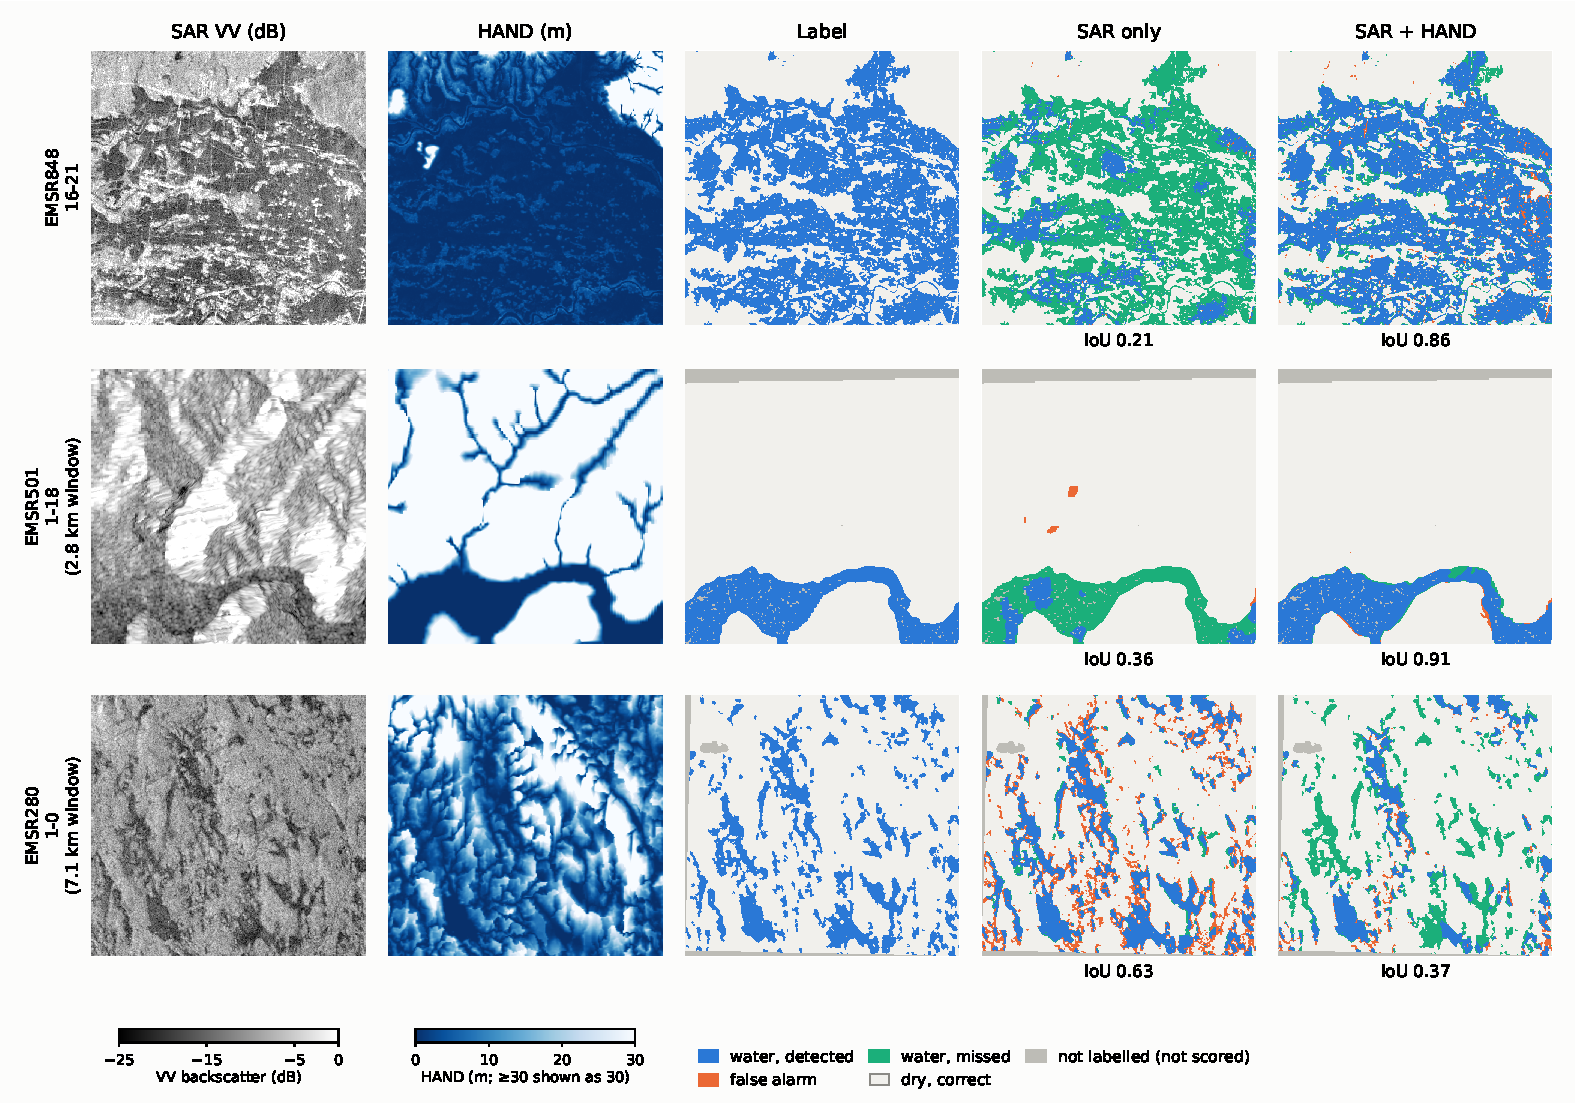
\includegraphics[width=\textwidth]{fig_example_tiles.pdf}
\caption{Example GEOID-Flood test tiles for the Sen1Floods11-trained U-Net (seed 0): SAR, HAND, label and
the errors of the SAR-only and SAR + HAND models. Top: floodplain gain; middle: mountain gain; bottom:
failure on Swedish lakes that sit above the DEM's drainage network (tile EMSR280\_1-0). Rows show windows of
different size (labelled; full 10.24-km tile in the top row), cropped to the labelled area; IoU is computed
over the whole tile.}
\label{fig:tiles}
\end{figure*}

\subsection{HAND, not just relief or known water}
\label{sec:ablation}

\begin{table}[t]
\caption{Which terrain helps in the Sen1Floods11 → GEOID-Flood transfer (pre-registered; trained on 11
events, 3 seeds; all 77/79 test events; two-way 95\% CIs).}
\label{tab:transfer_ablation}
\centering
\resizebox{\columnwidth}{!}{%
\begin{tabular}{@{}lccc@{}}
\toprule
Comparison & Flood, event-mean Δ & All water, event-mean Δ & Protocol pooled Δ \\
\midrule
DEM + slope vs SAR & +0.008 [−0.011, +0.026] & +0.014 [−0.027, +0.048] & +0.044 [+0.010, +0.086] \\
HAND vs DEM + slope & +0.024 [+0.005, +0.048] & +0.047 [+0.010, +0.099] & +0.028 [−0.004, +0.066] \\
HAND + DEM + slope vs HAND & −0.004 [−0.012, +0.004] & −0.004 [−0.014, +0.006] & +0.002 [−0.008, +0.014] \\
\bottomrule
\end{tabular}}
\end{table}

Is the transfer gain specific to HAND, or would any terrain input do? We fixed this test before training:
the same U-Net with DEM and slope instead of HAND, and with all three (Table~\ref{tab:transfer_ablation},
Fig.~\ref{fig:overview}b). DEM and slope recover only about a quarter of HAND's event-mean flood gain
(+0.008, CI including zero, against +0.032) and little of its all-water gain, and HAND beats them on both,
clearly for all water (+0.047 \ci{+0.010}{+0.099}, 68 of 79 events) and, for flood extent, with a CI close
to zero (+0.024 \ci{+0.005}{+0.048}, 55 of 77). Pooled over all pixels, which weights large events, DEM
and slope do better (+0.044 of HAND's +0.072 under the protocol): relief alone helps on the largest
floods, while HAND's drainage structure is what helps across events. Adding DEM and slope to HAND changes
nothing.

This differs from GEOID-Flood training (Table~S2). Trained on 20 GEOID-Flood events, DEM and slope recover
about two-thirds of HAND's flood gain (+0.021 vs.\ +0.032) and nine-tenths of its all-water gain, and HAND's
edge over them (+0.009 to +0.015 at 20 events) is not significant; at 159 events none of the terrain inputs changes flood
extent.

\emph{Not a permanent-water map.} A JRC Global Surface Water~\cite{pekel2016gsw} permanent-water channel
(occurrence ≥ 50\%, built identically for training and test; it reproduces Sen1Floods11's own JRC layer
at IoU 0.91) gives a third of HAND's all-water gain in the transfer (CIs over test events: +0.020 \ci{+0.010}{+0.030}, 61/79)
and slightly lowers flood IoU (−0.005 \ci{−0.009}{−0.001}); HAND beats it on both (+0.041
\ci{+0.024}{+0.060} all water, +0.038 \ci{+0.023}{+0.054} flood). With GEOID-Flood training (Table~S2),
JRC matches HAND's all-water gain at 20 events but explains none of the flood gain, and at 159 events it
\emph{hurts} flood extent (−0.054 \ci{−0.089}{−0.024} event-mean, −0.078 pooled): pooled flood recall on
unseen activations falls from 0.69 to 0.57 at unchanged precision (0.73 → 0.74). We read this as a shortcut:
the model learns that water is where the map says water already is and misses new flood water, which a
static water map invites and HAND, which marks where water \emph{could} collect, does not.

\subsection{The gain needs correctly located, detailed HAND}
\label{sec:mechanism}

\begin{table}[t]
\caption{HAND gain over SAR only when the HAND input is perturbed (pre-registered; Sen1Floods11-trained
U-Net, 3 seeds; all 77/79 GEOID-Flood test events; event-mean IoU, two-way 95\% CIs). Scored pixels are
identical in every row.}
\label{tab:mechanism}
\centering
\resizebox{\columnwidth}{!}{%
\begin{tabular}{@{}lcc@{}}
\toprule
HAND given to the model & Flood, Δ vs SAR only & All water, Δ vs SAR only \\
\midrule
Correct HAND & +0.032 [+0.018, +0.050] & +0.061 [+0.040, +0.086] \\
Shifted 100 m in x and y & +0.025 [+0.012, +0.041] & +0.031 [+0.012, +0.052] \\
Shifted 500 m in x and y & +0.003 [−0.011, +0.018] & −0.003 [−0.019, +0.013] \\
Blurred, $\sigma$ = 250 m & −0.001 [−0.015, +0.014] & −0.034 [−0.058, −0.010] \\
Another event's HAND (test only) & −0.061 [−0.081, −0.041] & −0.122 [−0.151, −0.095] \\
Another event's HAND (training and test) & −0.005 [−0.015, +0.006] & −0.001 [−0.021, +0.015] \\
\bottomrule
\end{tabular}}
\end{table}

Beating DEM and slope does not by itself show that the model uses what HAND says about the scene: the gain
could come from normalization, regularization or an easy-to-learn extra channel. We therefore fixed four
perturbations of the HAND input and one training control before running them (Table~\ref{tab:mechanism}).
Both hypotheses were supported. With HAND from a tile of another event the trained model becomes much worse
than SAR only (flood −0.061, all water −0.122), so it relies on HAND's content; shifted by 500\,m in both
axes (about 700\,m), the event-level gain disappears (+0.003 flood, −0.003 all water). A model trained and tested with another
event's HAND, which sees realistic HAND values that carry no information about the scene, gains nothing
(−0.005 \ci{−0.015}{+0.006} flood): the gain is not a side effect of having a terrain-like channel. A
100-m misregistration keeps most of the flood gain (+0.025) but halves the all-water gain, and blurring
away detail below about 250\,m removes the gain, so fine drainage structure matters. Pooled over all pixels,
the 500-m shift keeps about two-thirds of the flood gain (+0.050 \ci{+0.020}{+0.083} of +0.074; Table~S9), as large low-lying
areas stay low after a shift. Together with Table~\ref{tab:transfer_ablation}, this indicates that the gain comes
from correctly located, spatially detailed height above drainage across events, not from the extra
channel and not only from relief, which helps mainly on the largest low-lying floods.

\subsection{A foundation model does not replace terrain}
\label{sec:fm}

Does a large pretrained encoder make terrain redundant? We fine-tune TerraMind-1.0-base
\cite{jakubik2025terramind} (an 86\,M-parameter vision-transformer encoder pretrained on
TerraMesh~\cite{terramesh}, which includes Sentinel-1 GRD) with the U-Net decoder of the authors'
Sen1Floods11 configuration in TerraTorch~\cite{terratorch} (encoder layers 2, 5, 8 and 11; 101\,M
parameters in total, against 7.8\,M for our U-Net). VV and VH enter through the pretrained Sentinel-1 patch
embedding, standardized with TerraMind's own statistics; HAND enters as an extra band whose patch weights
start from random initialization, so the pretrained weights for VV and VH are unchanged. The learning
rate ($5\cdot10^{-5}$, from $2\cdot10^{-5}$, $5\cdot10^{-5}$ and $10^{-4}$) was chosen on the validation IoU
of the SAR-only model on one 20-event GEOID-Flood draw and reused unchanged for all TerraMind runs; all
other settings, data and step budgets equal the U-Net runs.

\begin{table}[t]
\caption{TerraMind ± HAND trained on the 11 Sen1Floods11 events (pre-registered; 3 seeds; all 77/79
GEOID-Flood test events; two-way 95\% CIs). TM: TerraMind-1.0-base, fine-tuned.}
\label{tab:fm_s1}
\centering
\resizebox{\columnwidth}{!}{%
\begin{tabular}{@{}lccc@{}}
\toprule
Comparison & Flood, event-mean Δ & All water, event-mean Δ & Protocol pooled Δ \\
\midrule
TM + HAND − TM & +0.031 [−0.000, +0.066] & +0.040 [+0.004, +0.081] & +0.026 [−0.009, +0.069] \\
TM − U-Net (SAR only) & −0.013 [−0.046, +0.018] & +0.009 [−0.030, +0.048] & +0.038 [−0.017, +0.094] \\
U-Net + HAND − TM & +0.045 [+0.022, +0.075] & +0.052 [+0.024, +0.087] & +0.034 [+0.005, +0.069] \\
\bottomrule
\end{tabular}}
\end{table}

In the main transfer setting (Table~\ref{tab:fm_s1}, Fig.~\ref{fig:overview}b), HAND helps TerraMind about
as much as it helps the U-Net in flood extent (+0.031 vs.\ +0.032 event-mean, the CI just reaching zero;
+0.036 \ci{+0.006}{+0.075} under the protocol, event-mean) and somewhat less for all water (+0.040 vs.\
+0.061). Without HAND, TerraMind is no better than the plain U-Net, and the 7.8\,M-parameter U-Net with HAND
beats it in all three measures of Table~\ref{tab:fm_s1} (flood +0.045 \ci{+0.022}{+0.075}, all water +0.052
\ci{+0.024}{+0.087}). With few training events, pretraining does not substitute for terrain in this configuration. These
comparisons use one fine-tuning setup (base model, U-Net decoder, one learning rate, HAND as an extra
patch-embedded band); more tuning or other fusion designs could change the ranking.

With GEOID-Flood training (Table~S3, Fig.~S3) the picture is similar: at 20 events HAND helps TerraMind
about as much as the U-Net in flood IoU (+0.031 vs.\ +0.032; both CIs only just exclude zero), less under
the protocol (+0.040 vs.\ +0.066), and not at 159 events. Our GEOID-trained TerraMind scores 0.491 under the
protocol on all 77 test events, slightly above GEOID-Flood's own TerraMind-B (0.478 frozen, 0.479
fine-tuned) and best single-image Sentinel-1 model (0.484).


\subsection{With 159 training events, HAND's flood-extent gain is not detectable}
\label{sec:geoid}

\begin{table*}[t]
\caption{Trained on GEOID-Flood train (159 events, 8,712 tiles, 3 seeds). Event-mean and pooled IoU,
SAR → SAR + HAND, with two-way 95\% CIs over seeds and test events.}
\label{tab:geoid}
\centering
\footnotesize
\begin{tabular}{@{}lccccc@{}}
\toprule
Test set & Events & Event-mean IoU & Δ (95\% CI) & Pooled IoU & Δ (95\% CI) \\
\midrule
GEOID test, unseen activations, all water & 39 & 0.625 → 0.648 & +0.023 [+0.004, +0.045] & 0.713 → 0.763 & +0.050 [+0.003, +0.118] \\
GEOID test, unseen activations, flooded only & 38 & 0.381 → 0.380 & −0.001 [−0.019, +0.016] & 0.549 → 0.559 & +0.011 [−0.017, +0.037] \\
GEOID test, shared activations, flooded only & 39 & 0.321 → 0.326 & +0.005 [−0.008, +0.024] & 0.468 → 0.438 & −0.030 [−0.059, −0.002] \\
GEOID held-out 2026, flooded only & 9 & 0.488 → 0.481 & −0.008 [−0.022, +0.007] & 0.644 → 0.626 & −0.017 [−0.034, +0.014] \\
Sen1Floods11 minus overlapping events & 8 & 0.512 → 0.530 & +0.018 [+0.008, +0.030]$^\dagger$ & 0.571 → 0.590 & \\
\bottomrule
\end{tabular}
\\[2pt]\raggedright\footnotesize $^\dagger$CI resamples test events only.
\end{table*}

Trained on GEOID-Flood's 159 training events, the picture changes (Table~\ref{tab:geoid}). This endpoint
differs from the 11-event one in training data (GEOID-Flood rather than Sen1Floods11) and in test events
(the 38/39 unseen activations rather than all 77/79), not only in the number of events; the learning curve
below varies the event count within GEOID-Flood. On flood
extent, HAND does nothing on unseen activations on either metric (event-mean −0.001, pooled +0.011, both
CIs include zero); threshold-free, flood AP is unchanged too (event-mean −0.000 \ci{−0.014}{+0.012}, CI over test events). On
all water it still helps, though with CIs close to zero (+0.023 \ci{+0.004}{+0.045} event-mean, +0.050
\ci{+0.003}{+0.118} pooled). On test activations that share AoIs with training, HAND \emph{lowers} pooled
flood IoU (0.468 → 0.438) while event-mean IoU is unchanged; one event, EMSR419, dominates
(Section~\ref{sec:failures}).

Under the GEOID-Flood protocol our GEOID-trained U-Net scores \iouf{} 0.452 ± 0.005 (SAR) and 0.469 ±
0.008 (+ HAND) on the 77 test events with flood, inside the 0.41--0.48 that GEOID-Flood reports for
single-image Sentinel-1 models with ImageNet or foundation-model encoders (one frozen encoder, Satlas,
scores 0.21), so our pipeline and baselines are comparable. HAND's protocol gain at 159 events is small,
with a CI just above zero on all 77 events (+0.017 \ci{+0.001}{+0.035}) and including zero on unseen
activations alone (+0.021 \ci{−0.001}{+0.043}). Scoring the post-event map alone against flood labels,
with permanent water as a false positive, instead gives −0.009 \ci{−0.021}{−0.000} on all 77 events
(−0.008 \ci{−0.024}{+0.007} on unseen activations): the protocol gain comes from better water detection in
both images, which the pre-image subtraction turns into flood IoU, not from better flood delineation. On
the nine held-out 2026 events the protocol gain is −0.017 \ci{−0.039}{+0.018}.

\begin{figure}[t]
\centering
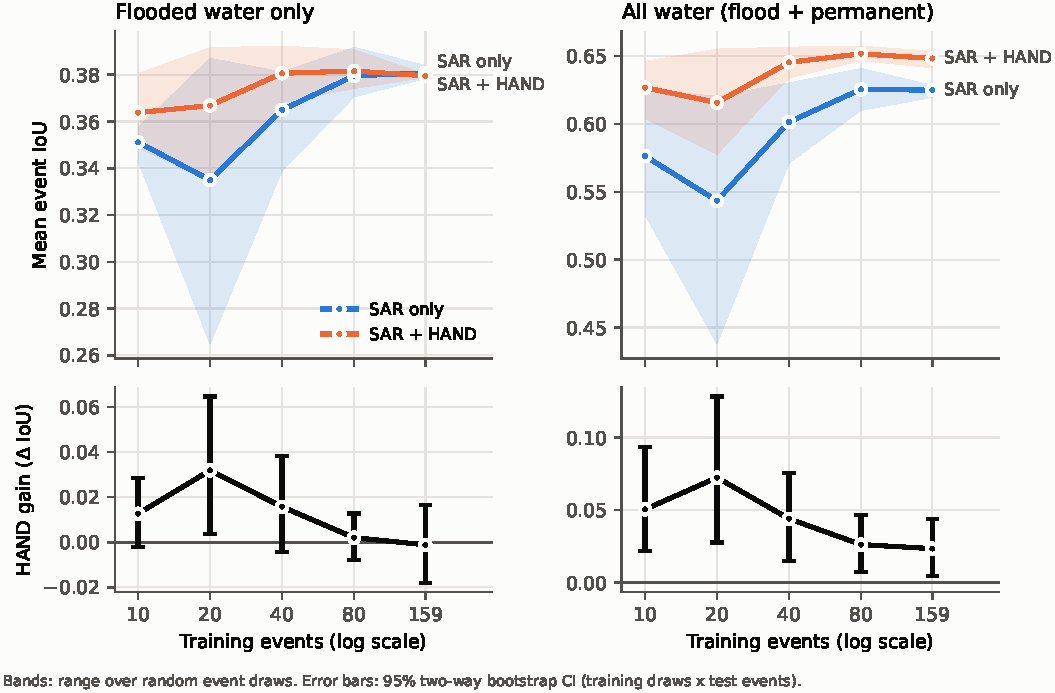
\includegraphics[width=\columnwidth]{fig_learning_curve.pdf}
\caption{IoU and HAND gain against the number of GEOID-Flood training events (unseen test activations,
event-mean IoU). Top: mean over draws, band = range over draws. Bottom: HAND gain with two-way 95\% CIs
over draws and test events.}
\label{fig:curve}
\end{figure}

\begin{table}[t]
\caption{HAND gain against the number of GEOID-Flood training events, flooded water only, 38 unseen test
activations (5 draws; 159 events: 3 seeds). Two-way 95\% CIs.}
\label{tab:curve}
\centering
\resizebox{\columnwidth}{!}{%
\begin{tabular}{@{}lccc@{}}
\toprule
Training events (tiles) & Event-mean Δ & Pooled IoU, SAR → + HAND & Pooled Δ \\
\midrule
10 (262–728) & +0.013 [−0.002, +0.028] & 0.490 → 0.529 & +0.039 [+0.008, +0.070] \\
20 (651–1,759) & +0.032 [+0.004, +0.065] & 0.468 → 0.530 & +0.062 [+0.019, +0.111] \\
40 (1,834–3,168) & +0.016 [−0.004, +0.038] & 0.513 → 0.561 & +0.048 [+0.015, +0.083] \\
80 (3,387–4,827) & +0.002 [−0.008, +0.012] & 0.539 → 0.561 & +0.022 [−0.002, +0.052] \\
159 (8,712) & −0.001 [−0.019, +0.016] & 0.549 → 0.559 & +0.011 [−0.017, +0.037] \\
\bottomrule
\end{tabular}}
\end{table}

\emph{Learning curve.} To see how the value of HAND depends on the number of training events, we train on
random subsets of 10, 20, 40 and 80 GEOID-Flood training events (5 draws each; draw $k$ trained with seed
$k$) and on the full 159, all with the same step budget (Fig.~\ref{fig:curve}, Table~\ref{tab:curve}).
Exploratory, the flood-extent HAND gain looked largest at 20--40 events and gone by 159: at 20 events its
CI only just excludes zero (+0.032 \ci{+0.004}{+0.065}), at 40 the pooled CI excludes zero but the
event-mean one does not, and at 80 both include zero. Which events are in a small training set matters:
at 20 events the per-draw flood gain ranges from −0.008 to +0.069. With HAND, 20 events approach the pooled
flood IoU that SAR-only reaches with 80--159 (0.530 vs.\ 0.539--0.549).

\emph{The pre-registered confirmation failed.} To test the decline, we fixed a contrast before training
new models: on three new, independent equal-tiles draws (500 tiles) at each of 20, 40 and 159 events, the
mean HAND gain at 20 and 40 events minus the gain at 159, on the 38 unseen test events, with a one-sided
Wilcoxon test over events. The contrast was +0.0025 \ci{−0.007}{+0.013} (CI over test
events), $p = 0.37$ (all water $p = 0.37$), against +0.012 \ci{+0.004}{+0.019}, $p = 0.003$, on the
exploratory draws that motivated it; a post hoc average-precision version is also null ($p = 0.49$; details
with Table~S4). We therefore do not claim that the HAND gain declines steadily with event count; the robust
statements are the endpoints---a clear gain when training on 11 Sen1Floods11 events and testing
externally, and no detectable flood-extent gain with 159 GEOID-Flood events.

\emph{Events, not tiles.} A control cuts every subset to exactly 500 tiles spread evenly over its events
(3 draws; Table~S4, Fig.~S1). 500 tiles from all 159 events match all 8,712 for the SAR-only model (flood
event-mean 0.381 vs.\ 0.381; all water 0.632 vs.\ 0.625). Because the step budget is fixed and each subset
has different events, this shows that extra tiles from the same events add nothing at this budget; it does
not isolate event diversity as a cause. Regressing event-mean IoU on log events and log
tiles over all 38 exploratory draws (Table~S5), the SAR-only model improves with each doubling of events
(flood +0.007 \ci{+0.001}{+0.015}, all water +0.014 \ci{+0.004}{+0.028}; suggestive by our criterion) and
not with more tiles (−0.001 and −0.004, CIs including zero).

\subsection{The pre-event image partly substitutes for terrain}
\label{sec:cd}

GEOID-Flood provides a pre-event Sentinel-1 image for every tile, so a model can be given both images at
once. Operationally, Sentinel-1's routine acquisitions usually supply a recent pre-event image of the same
orbit, but seasonal changes in vegetation and soil moisture between the two dates add their own errors. We train the same U-Net on [VV, VH, VV\textsubscript{pre}, VH\textsubscript{pre}] (± HAND) to predict
flooded water directly, with permanent water and background as negatives, i.e., GEOID-Flood's flood class.
All 8,712 training tiles have a pre-event image; requiring both images removes 0.8\% of valid pixels. It
is scored on exactly the tiles and pixels of the protocol-matched single-image numbers, so the rows of
Table~\ref{tab:cd} are directly comparable.

\begin{table}[t]
\caption{HAND gain with and without the pre-event image (unseen activations; pooled \iouf{} under the
GEOID-Flood protocol, mean over draws/seeds; Δ from confusion counts averaged over draws/seeds, two-way
95\% CI; last column event-mean Δ).}
\label{tab:cd}
\centering
\footnotesize
\setlength{\tabcolsep}{2.5pt}
\resizebox{\columnwidth}{!}{%
\begin{tabular}{@{}lccccc@{}}
\toprule
Model & Events & SAR & + HAND & Δ pooled (95\% CI) & Δ ev. \\
\midrule
Single image, differenced & 20 & 0.382 & 0.448 & +0.066 [+0.019, +0.111] & +0.036 \\
Change detection & 20 & 0.404 & 0.426 & +0.024 [−0.037, +0.085] & +0.000 \\
Single image, differenced & 159 & 0.475 & 0.496 & +0.021 [−0.001, +0.043] & +0.013 \\
Change detection & 159 & 0.463 & 0.491 & +0.029 [−0.011, +0.057] & +0.005 \\
\bottomrule
\end{tabular}}
\end{table}

A trained change model is no better than differencing two single-image maps (without HAND: −0.014
\ci{−0.069}{+0.037} at 159 events, +0.020 \ci{−0.048}{+0.098} at 20), but it is much less sensitive to
which 20 events it is trained on (standard deviation over draws 0.041 vs.\ 0.090). With the pre-event
image, HAND matters less at 20 events (+0.024 vs.\ +0.066, no longer significant) and about as much at 159
(+0.029 vs.\ +0.021); the event-mean gains are near zero. Plausibly the pre-event image supplies part of what
HAND supplies with few training events: which dark, smooth surfaces were already there before the flood.

\subsection{Failure cases resist two pre-registered remedies}
\label{sec:failures}

HAND fails in two ways. On flat ground where every pixel is near drainage it pushes the model toward flood
everywhere: Somalia in LOEO, and EMSR419 (Iran, January 2020) with GEOID-Flood training, whose tiles have a
median HAND of 0.44\,m with 81\% of pixels below 2\,m (5.8\,m and 38\% over the test set) and which
contributes 1.37\,M of the 1.56\,M extra false-positive pixels on shared activations (event IoU 0.188 →
0.142). And it suppresses water bodies the DEM drainage network misses: on a Swedish tile
(EMSR280\_1-0; Fig.~\ref{fig:tiles}, bottom) HAND suppresses lakes that sit above the network (tile IoU
0.61 → 0.30 over 3 seeds), although over the whole Swedish event (113 tiles) HAND still helps (0.548 →
0.663).

\emph{Relief gate.} The obvious remedy for the first failure is to ignore HAND on flat ground. We fixed the
rule before computing any outcome: a tile is \emph{flat} when the 90th percentile of its valid HAND is below
2\,m, and flat tiles take the SAR-only model's prediction from the same seed or draw (5\% of test tiles, in
28 of 80 events; no retraining or tuning). The primary outcome, pooled \iouf{} under the protocol on
unseen activations, does not improve (gated minus ungated: −0.016 \ci{−0.047}{+0.001} at 20 events, −0.003
\ci{−0.007}{+0.001} at 159; Table~S6), and on all 77 test events at 20 training events the gate lowers it
(−0.012 \ci{−0.030}{−0.001}). Gating more tiles costs more (exploratory: threshold 5\,m −0.022
\ci{−0.053}{−0.002}): HAND helps on flat tiles on average, and the failure is concentrated in a few events,
not a property of flat tiles.

\emph{HAND dropout.} For the second failure, which puts real water at high HAND, a standard remedy is
modality dropout~\cite{neverova2016moddrop}: during training the HAND channel of a random 50\% of tiles is
replaced by −1 (outside the normalized range), and HAND is always present at test time. Fixed before
training (Table~S7), it does not help: dropout raises no mean gain by more than +0.001, and with 11 training
events it removes a quarter to two-fifths of HAND's gain over SAR only (flood event-mean −0.008
\ci{−0.016}{−0.001}, all water −0.020 \ci{−0.036}{−0.009}). At 159 events it shrinks the model toward SAR
only: fewer large losses (protocol tail 5 → 2 events) but also fewer gains (events improved 25 → 21). The
Swedish tile recovers partly (0.30 → 0.46), but the Swedish event as a whole gets worse in every setting,
because HAND helps most of that event's tiles.
